\subsection{Realimentación}
La ilustración \ref{ilus:amplificador-base} muestra el modelo dinámico del amplificador base. Cuyos parámetros son los mostrados en la tabla \ref{tab:amplificador-base-dinamico}.

\begin{ilustracion}[ht]
    \centering
    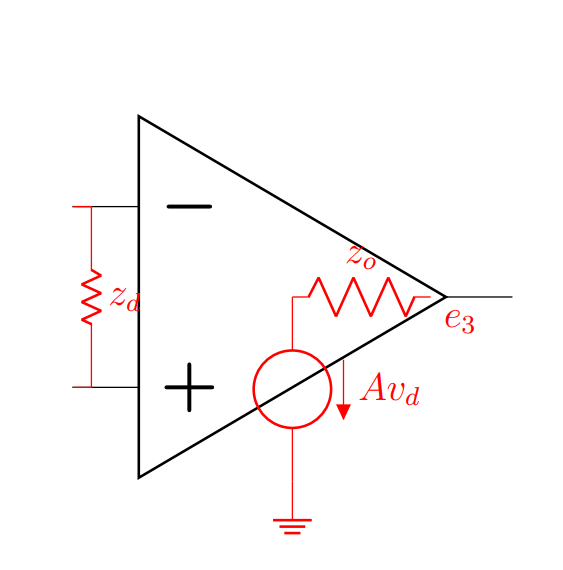
\includegraphics[width=0.6\textwidth]{src/images/p5/modelo-amplificador.png}
    \caption{Modelo dinámico del amplificador base}
    \label{ilus:amplificador-base}
\end{ilustracion}
Ahora calculamos los parámetros del amplificador realimentado negativamente.

para la impedancia de entrada $Z_i$ tenemos:

$$Z_i = R_s = 3.3 k\Omega$$

Y la impedancia de salida viene dada por la expresión:

$$Z_o = \frac{R_o}{A / (1 + \frac{R_f}{R_s})}$$

Por lo tanto el valor de $Z_o$ es:

$$Z_o = 0.137 \Omega$$

El valor de la ganancia de la realimentación negativa es: 

$$A_{fb} = - \frac{R_f}{R_s} = - \frac{11k\Omega}{3.3k\Omega} = -3.33$$

Y debido a que $A => \infty$ en el amplificador base, el valor de la ganancia de la realimentación negativa es:

$$A = -\frac{1}{\beta}$$

despejando $\beta$ de la expresión anterior, tenemos:

$$\beta = -\frac{1}{A} = -\frac{1}{3.33} = 0.333$$

Para encontrar las frecuencias de corte inferior utilizamos la expresión:

$$f_{Lf} = \frac{f_{Lb}}{1 + A_{b}}$$

entonces:

$$f_{Hf} = \frac{69.61 Hz}{1 + 49.54} = 1.37 Hz$$

Para hallar la frecuencia de corte superior utilizamos la expresión:

$$f_{Hf} = f_{Hb}\cdot (1 + A_{b})$$

Por lo tanto:

$$f_{Hf} = 11kHz\cdot (1 + 49.54) = 555.94KHz$$

\begin{table}[ht]
    \centering
    \begin{tabular}{|c|c|c|c|}
        \hline
        \textbf{Parámetro} & \textbf{Valor} \\ \hline
        $Z_i$ & $3.3$ [$k\Omega$] \\ \hline
        $Z_o$ & $0.17 $ [$\Omega$] \\ \hline
        $A_b$ & $-3.33$ \\ \hline
        $f_L$ & $1.37$ [$Hz$] \\ \hline
        $f_H$ & $555.94$ [$kHz$] \\ \hline
    \end{tabular}
    \caption{Valores de los parámetros dinámicos del amplificador Realimentado}
    \label{tab:amplificador-base-dinamico}

\end{table}

Ahora, para el amplificador realimentado positivamente, procedemos a calcular la ganancia:

$$A_{fb} = 1 + \frac{R_f}{R_s} = 1 + \frac{11k\Omega}{3.3k\Omega} = 4.33$$

La impedancia de entrada con realimentación positiva es:

$$ Z_i = \frac{Z_d \cdot A_b}{1 + \frac{R_f}{R_s}} = \frac{43.99k\Omega \cdot 300}{1 + \frac{11k\Omega}{3.3k\Omega}} = 3.05M\Omega$$

Y la impedancia de salida con realimentación positiva es igual a la impedancia de salida de realimentación negativa:

$$Z_o = 0.137 \Omega$$

La ilustración \ref{ilus:amplificador-realimentado-negativo} muestra el circuito del amplificador realimentado negativamente construido en multisim.

\begin{ilustracion}[ht]
    \centering
    \includegraphics[width=1.0\textwidth]{src/images/p5/Prelaboratorio 5 - Realimentación negativa - circuito.png}
    \caption{Circuito amplificador con realimentación negativa}
    \label{ilus:amplificador-realimentado-negativo}
\end{ilustracion}
\FloatBarrier

En la ilustración \ref{ilus:ganancia-realimentacion-negativa} podemos observar una ganancia de aproximadamente $3.3$ que coincide con la ganancia de los cálculos.

\begin{ilustracion}[ht]
    \centering
    \includegraphics[width=1\textwidth]{src/images/p5/Prelaboratorio 5 - Retroalimentación negativa - Ganancia.png}
    \caption{Ganancia de la realimentación negativa}
    \label{ilus:ganancia-realimentacion-negativa}
\end{ilustracion}

En la ilustración \ref{ilus:respuesta-frecuencia-realimentacion-negativa} podemos observar un aumento en el ancho de banda con realimentación negativa. Podemos observar que las frecuencias de corte coinciden con los cálculados previamente.

\begin{ilustracion}[ht]
    \centering
    \includegraphics[width=1.0\textwidth]{src/images/p5/Prelaboratorio 5 - retroalimentación negativa - respuesta en frecuencia.png}
    \caption{Respuesta en frecuencia del amplificador realimentado negativamente}
    \label{ilus:respuesta-frecuencia-realimentacion-negativa}
\end{ilustracion}
\FloatBarrier

% Realimentación positiva

La ilustración \ref{ilus:circuito-realimentacion-positiva-sin-condensador} muestra la construcción del circuito del amplificador realimentado positivamente.

\begin{ilustracion}[ht]
    \centering
    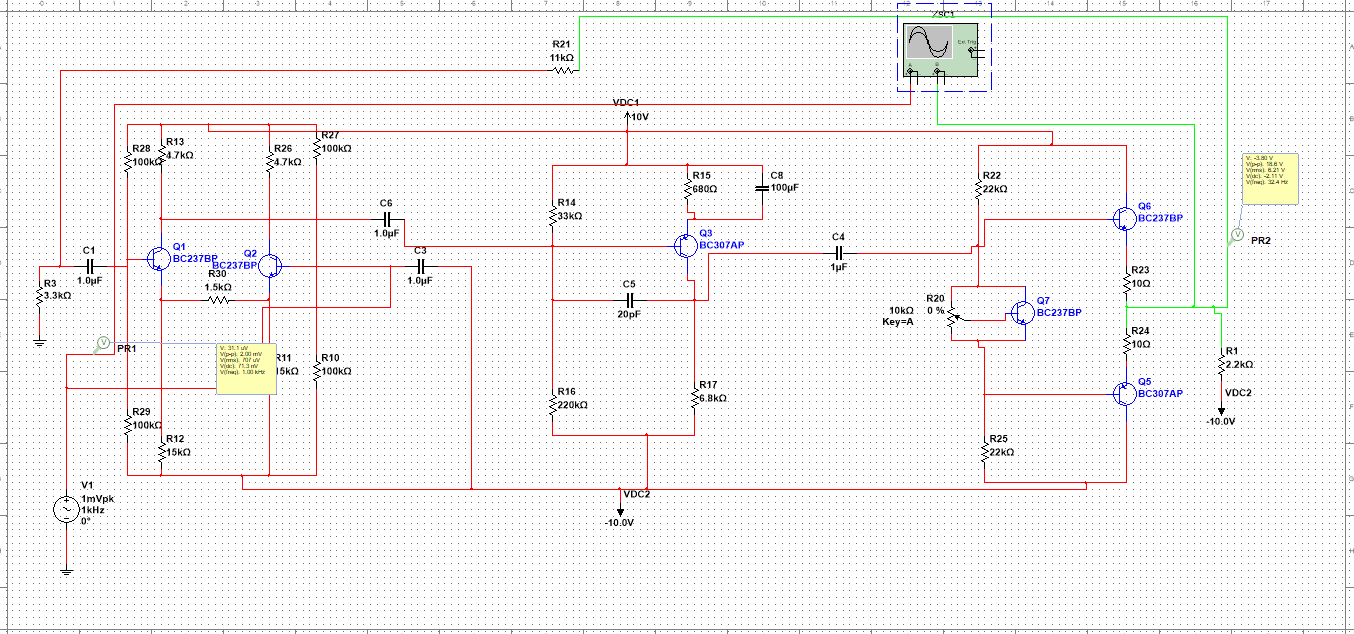
\includegraphics[width=\textwidth]{src/images/p5/Prelaboratorio 5 - Realimentacion positiva sin condensador - circuito.png}
    \caption{Circuito de realimentación positiva sin condensador}
    \label{ilus:circuito-realimentacion-positiva-sin-condensador}
\end{ilustracion}

La ganancia de este amplificador se puede observar en la ilustración del \ref{ilus:ganancia-circuito-realimentacion-positiva-sin-condensador} y podemos observar que coincide con la ganancia calculada anteriormente de 4.33. Sin embargo podemos observar que despues de un tiempo la ganancia cambia y toma la forma mostrada en la ilustración \ref{ilus:ganancia-circuito-realimentacion-positiva-sin-condensador-despues-de-unos-segundos}.

\begin{ilustracion}[ht]
    \centering
    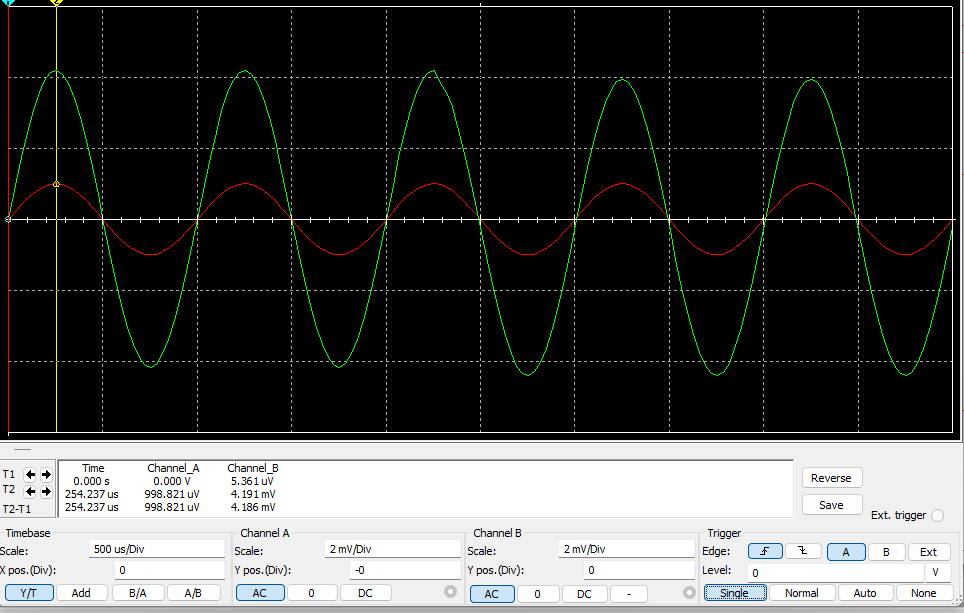
\includegraphics[width=\textwidth]{src/images/p5/Prelaboratorio 5 - Realimentacion positiva sin condensador - ganancia.png}
    \caption{Ganancia del circuito de realimentación positiva sin condensador}
    \label{ilus:ganancia-circuito-realimentacion-positiva-sin-condensador}
\end{ilustracion}
\FloatBarrier


\begin{ilustracion}[ht]
    \centering
    \includegraphics[width=\textwidth]{src/images/p5/Prelaboratorio 5 - Retroalimentación positiva sin condensador despues de unos segundos.png}
    \caption{Ganancia del circuito de realimentación positiva sin condensador despues de unos segundos}
    \label{ilus:ganancia-circuito-realimentacion-positiva-sin-condensador-despues-de-unos-segundos}
\end{ilustracion}
\FloatBarrier

Podemos observar la respuesta en frecuencia del amplificador realimentado positivamente en la ilustración \ref{ilus:respuesta-amplificador-realimentacion-positiva-sin-condensador}.

\begin{ilustracion}[ht]
    \centering
    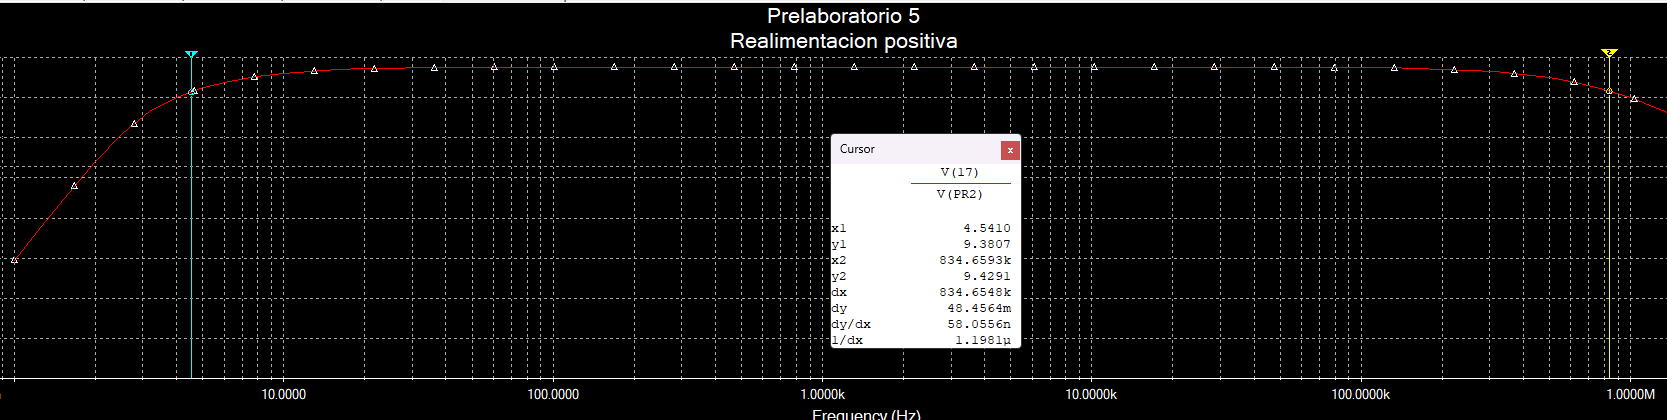
\includegraphics[width=\textwidth]{src/images/p5/Prelaboratorio 5 - realimentacion positiva sin condensador - respuesta en frecuencia.png}
    \caption{Respuesta en frecuencia del amplificador con Realimentación positiva sin condensador} 
    \label{ilus:respuesta-amplificador-realimentacion-positiva-sin-condensador}
\end{ilustracion}

Amplificador realimentado positiva y negativamente

La ilustración \ref{ilus:circuito-amplificador-realimentacion-positiva-y-negativa} muestra el circuito del amplificador con realimentación positiva y negativa con condensador.

\begin{ilustracion}[ht]
    \centering
    \includegraphics[width=\textwidth]{src/images/p5/prelaboratorio 5 - circuito realimentación positiva con condensador.png}
    \caption{Circuito con realimentación positiva y negativa} 
    \label{ilus:circuito-amplificador-realimentacion-positiva-y-negativa}
\end{ilustracion}
\FloatBarrier

La ganancia este amplificador se puede observar en la ilustración \ref{ilus:ganancia-amplificador-realimentacion-positiva-y-negativa}.
\begin{ilustracion}[ht]
    \centering
    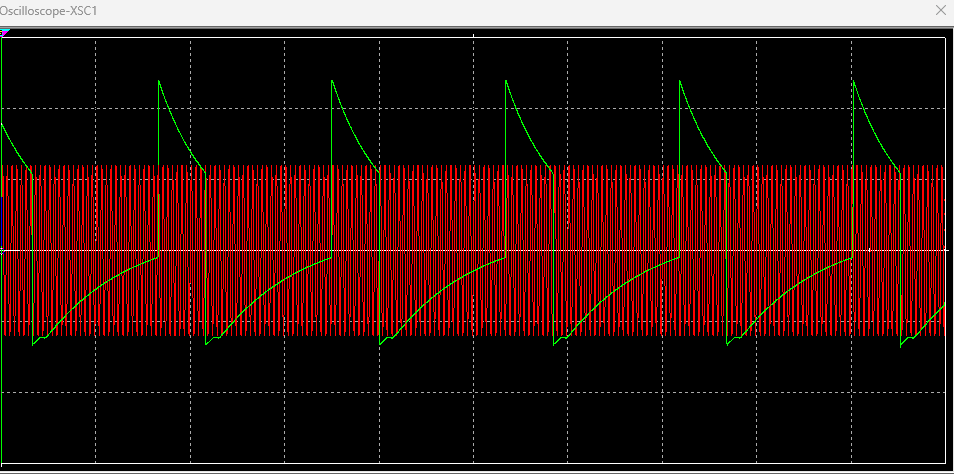
\includegraphics[width=\textwidth]{src/images/p5/Prelaboratorio 5 - Ganancia realimentacion positiva con condensador.png}
    \caption{Ganancia con realimentación positiva y negativa} 
    \label{ilus:ganancia-amplificador-realimentacion-positiva-y-negativa}
\end{ilustracion}
\FloatBarrier

La respuesta en frecuencia del amplificador se puede observar en la ilustración \ref{ilus:respuesta-amplificador-realimentacion-positiva-y-negativa}.

\begin{ilustracion}[ht]
    \centering
    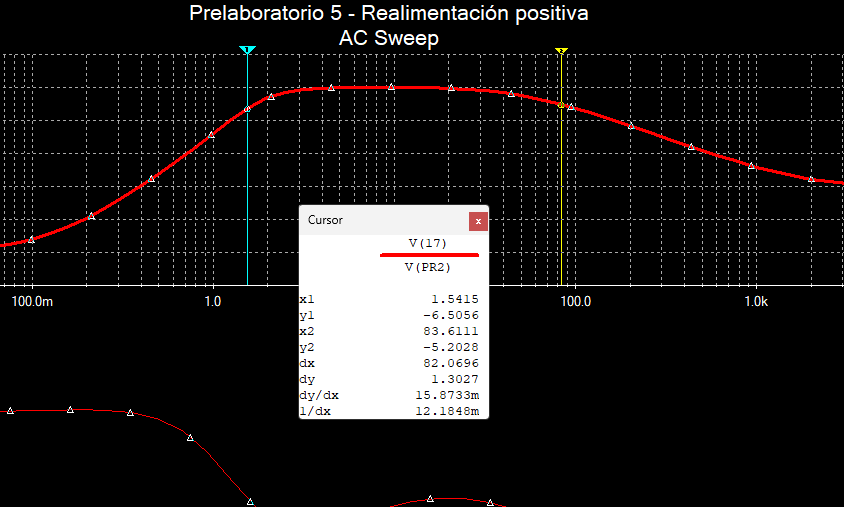
\includegraphics[width=\textwidth]{src/images/p5/Prelaboratorio 5 - Respuesta en frecuencia - realimentacion positiva con condensador.png}
    \caption{Circuito con realimentación positiva y negativa} 
    \label{ilus:respuesta-amplificador-realimentacion-positiva-y-negativa}
\end{ilustracion}
